\section{Reward, OLO, Optimization, and Automatic Model Selection}

\begin{figure}[t]
\centering
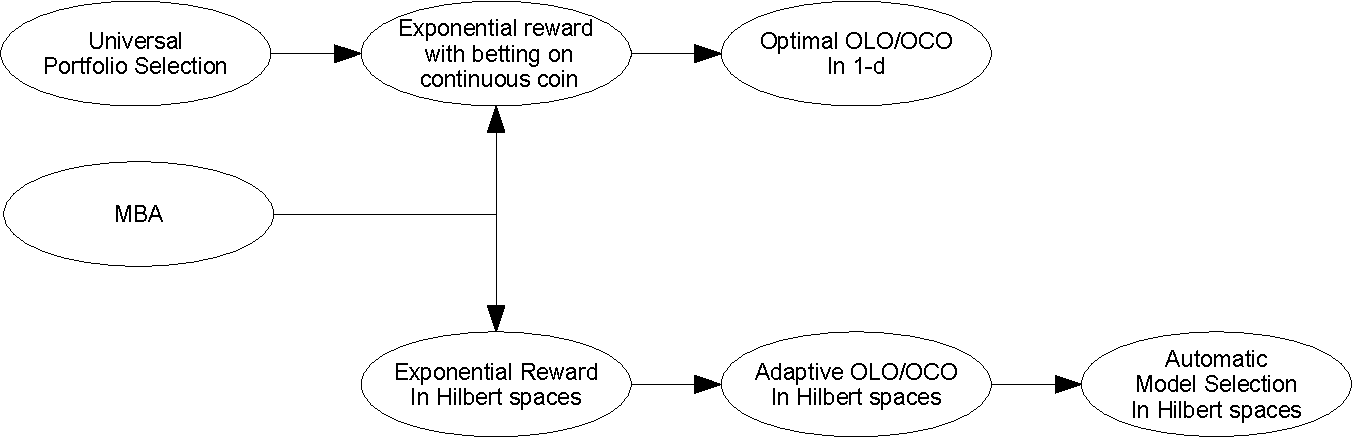
\includegraphics[width=.95\linewidth]{./figs/links_between_areas.pdf}
\caption{The links between the different areas and betting.}
\end{figure}

In this section we will show the connection between portfolio selection, betting on a continous coin, adaptive OLO, and automatic model selection. We will prove that, given an ``optimal'' betting algorithm, the same algorithm can be used to solve all the problems listed above.

\textbf{Betting vs. OLO.}
We use the duality between Regret and Reward in \citet{McMahanO14}.
We have the following Theorem.
\begin{theorem}
  \label{thm:rrdual}
  Let $\Psi:\mathcal{H} \rightarrow (-\inf, +\inf]$ be a lower semicontinuos and convex function, with $dom \Psi \neq \emptyset$. An
  algorithm for the player guarantees
  \[
  Reward \geq \Psi(-g_{1:n}) - \epsilon \quad \quad \quad \textnormal{ for any } g_1, \dots, g_n
  \]
  for a constant $\epsilon \in \R$ if and only if it
  guarantees
  \begin{equation}\label{eq:regb}
  \qquad Regret(u) \leq \Psi^*(u) + \epsilon \quad \quad \quad \textnormal{ for all } u \in \mathcal{H}~.
  \end{equation}
\end{theorem}

The above Theorem proves that the reward and regret view on online learning are equivalent: an algorithm guarantees low regret iff it guarantees high reward. Hence a betting algorithm can be used for online learning and vice-versa. However, as it was already stressed in \citet{McMahanO14}, the reward view has the big advantage of having one variable less, the competitor $\bu$.
Moreover, as we will show in Section~\ref{}, designing and analysing algorithms in one of the two views could be much easier than in the other one.

\textbf{OLO and Optimization.}
It is well known that a regret bound can be transformed into a convergence guarantee for optimization of convex functions.
In particular, we have the following Theorem from~\citet{Cesa-BianchiCG04}.
%
\begin{theorem}
Let $\bw_1, \cdots, \bw_n \in \fH$ the vector produced by an OLO algorithm $\mathcal{A}$ with a regret guarantee $R_A(n)$.
Let $F:\fH\rightarrow\R$ a convex function, and fix the vectors $\bg_t$ to be unbiased estimate of the gradient of $F$ in $\bw_t$. Then, the following holds
\[
\E\left[F\left(\frac{1}{n} \bw_t\right)\right] \leq \frac{\E[R_A(n)]}{n}~.
\]
\end{theorem}

High probability bounds can be also easily obtained, assuming more on the function $F$~\citep{Cesa-BianchiCG04}.
The above theorem says that, if the regret grows, for example, as $\scO(\sqrt{n})$, the OLO algorithm can be used as a stochastic optimization algorithm with convergence in expectation $\scO(\frac{1}{\sqrt{n}})$.

\textbf{Adaptive Algorithms for OLO and Self-tuning Model Selection.}
In learning theory a key concept is the one of regularization. If the concept class we are learning is too rich, we need to constrain the complexity of the trained predictor. A regularizer is achieving this, biasing the classifieres towards a small region of the space. However, it is known that the optimal amount of regularization is completely problem-dependent. Hence, the regularizer becomes another parameter to be learned.

Most, if not all, the machine learning algorithms uses a two-stages process to find the optimal amount of regularization. First, the algorithm is trained with a fixed regularization parameter. Second, its generalization performance is estimated together with a change in the regularization parameter. These two steps are repeated till convergence.

Surprisingly enough, \citep{Orabona14} proved that the above procedure can be avoided with a stochastic learner. In particular, instead of solving a series of regularized ERM problems, with different amounts of regularization, one can use a simple prarameter-free stochastic gradient descent procedure over the training samples and achieve the same performance.
More rigorously, the follwing theorem holds.
\begin{theorem}
Let $\bw_1, \cdots, \bw_n \in \fH$ the vector produced by the PiSTOL algorithm.
Let $\ell:\R\rightarrow\R$ a convex and Lipschitz function, and fix the vectors $\bg_t$ to be unbiased estimate of the gradient of $F$ in $\bw_t$. Then, the rate of convergence of $\E\left[Risk_F\left(\frac{1}{n} \bw_t\right)\right]$ is the same of regularized ERM algorithm with the (unknown) optimal amount of regularization.
\end{theorem}

Moreover, from \citep{} we can extract the following Theorem.
\begin{theorem}
When PiSTOL is used as a betting strategy against a coin with outcomes in $[-1,1]$, it guarantees an exponential reward.
\end{theorem}

In reality, the connection between betting and self-tuning regularized ERM is actually stronger. In fact, the following theorem can be proved.
\begin{theorem}
If a betting strategy against a coin with outcomes in $[-1,1]$ guarantees an exponential reward, the same algorith used for SGD over the risk of a convex loss will guarantee optimal rate of convergence to the Bayes risk.
\end{theorem}

To summarize, we have that regret minimization in OLO is equivalent to reward maximization. Moreover, optimal betting algorithms correspond to adaptive OLO algorithms, that guarantees automatic model selection when used in infinite dimensional spaces. In the next section we will explain what are the difficulties in designing an optimal betting strategy.